\chapter{Sonarqube}
Sonarqube wordt gebruikt voor het analyseren van de geschreven code van een applicatie. Om de code te analyseren zijn een aantal verschillende regels standaard ingebouwd in Sonarqube waar we gebruik van maken.
In de configuratie voor de Staging omgeving van de verschillende applicaties in Jenkins, is een extra "maven goal"\ toegevoegd die de integratie met Sonarqube verzorgd.

\section{Container configuratie}
Er waren weinig stappen vereist om Sonarqube in docker te kunnen draaien. Hetgeen wel belangrijk is, is om ervoor te zorgen dat Sonarqube van buitenaf bereikbaar is. Dit kunnen we doen door de twee poorten die Sonarqube gebruikt (9000 en 9092) open te zetten.

Aangezien de Portainer container reeds gebruikt maakt van poort 9000, is het van belang dat Sonarqube van een andere poort gebruikt maakt om van buitenaf bereikbaar te zijn. We hebben poort 9000 van Sonarqbue dan ook gemapped met poort 9001 voor de buitenwereld. Hierdoor vind er geen overlapping plaats in de poortconfiguratie met Portainer en Sonarqube.

\begin{figure}[H]
	\centering
	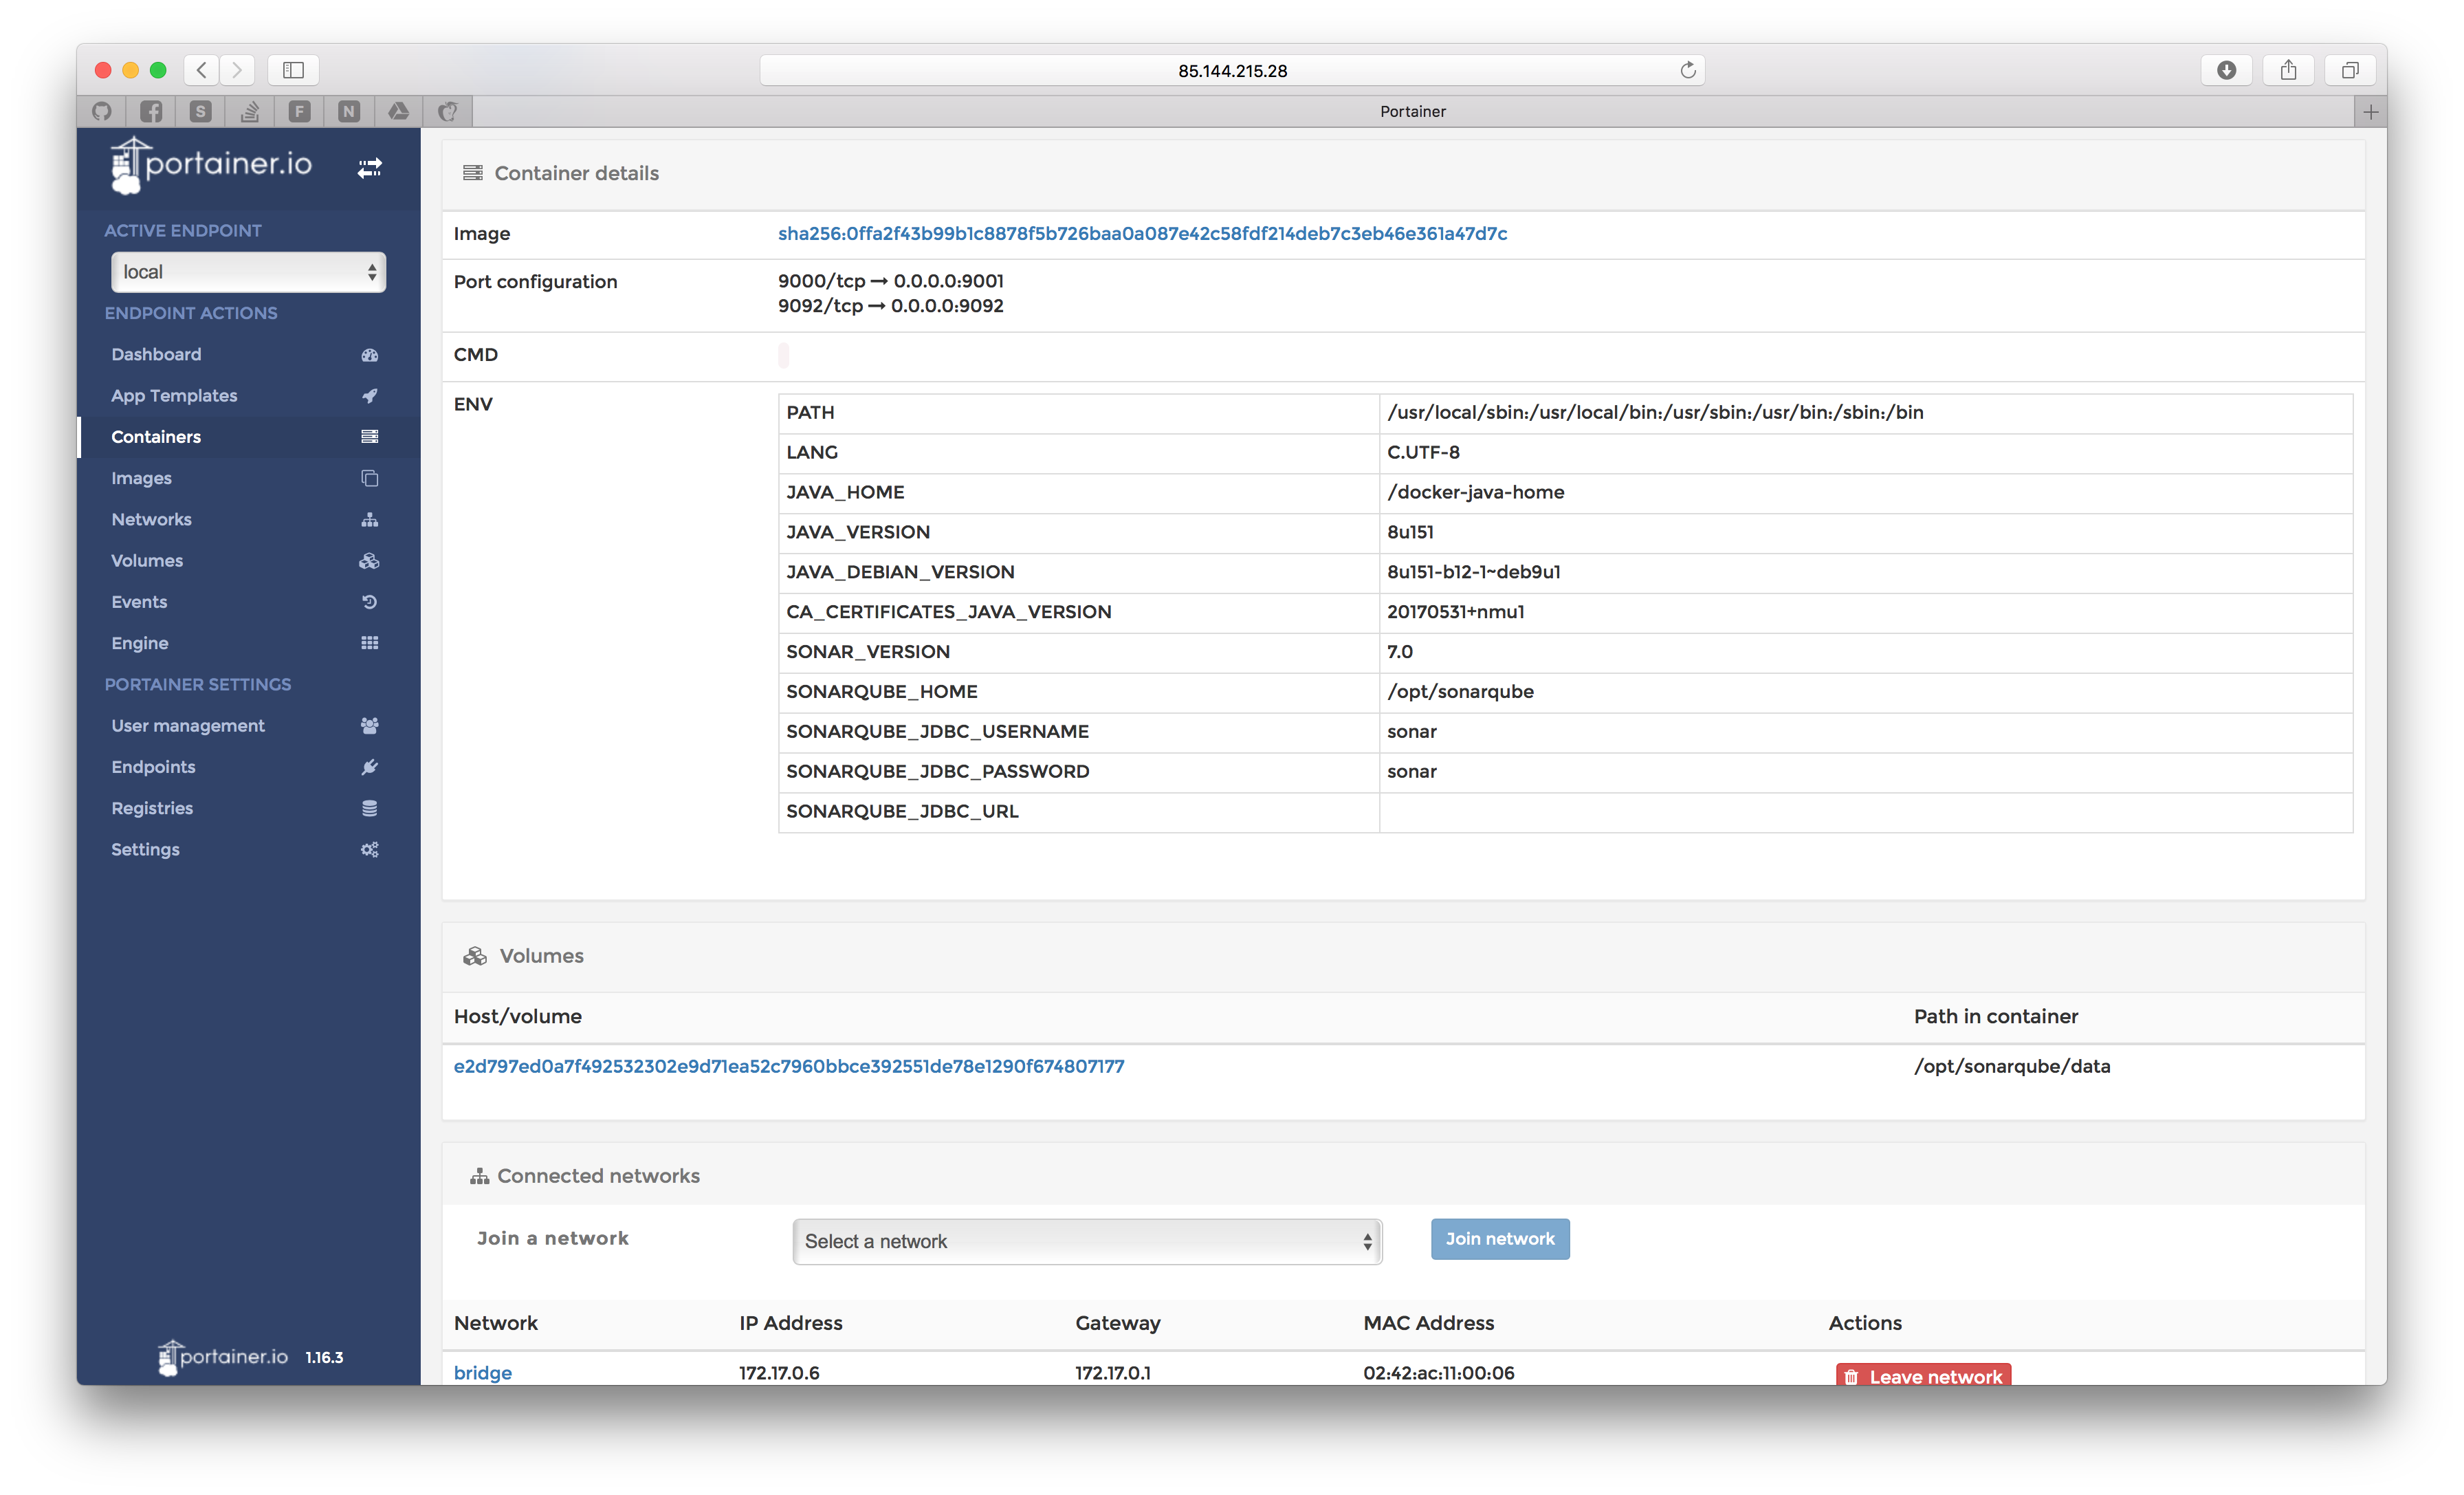
\includegraphics[width=0.95\textwidth]{img/SonarqubeContainerDetails.png}
	\caption{Container configuratie van Sonarqube}
	\label{fig:SonarqubeContainerDetails}
\end{figure}

\newpage
\section{Configuratie van Sonarqube voor projecten}
De configuratie van Sonarqube voor een project kunnen we automatisch laten uitvoeren door Jenkins. Zoals eerder vermeld kan de analyse van de code gestart worden door een "maven goal"\ op te geven: 
\begin{lstlisting}
sonar:sonar -Dsonar.host.url=http://85.144.215.28:9001 -Dsonar.login=XXX
\end{lstlisting}

\subsubsection{sonar.host.url}
Om de code van een project te analyseren, moet voor maven bekend zijn op welk adres Sonarqube bereikbaar is. We geven hierbij het IP adres waar Sonarqube op bereikbaar is op, inclusief poortnummer.
\subsubsection{sonar.login}
Wanneer een gebruiker ingelogd is op Sonarqube, kan hij/zij bij zijn account een nieuw token genereren. Dit (login) token moet gebruikt worden om verbinding te maken met Sonarqube wanneer maven de code wilt doorsturen om te analyseren.

\begin{figure}[H]
	\centering
	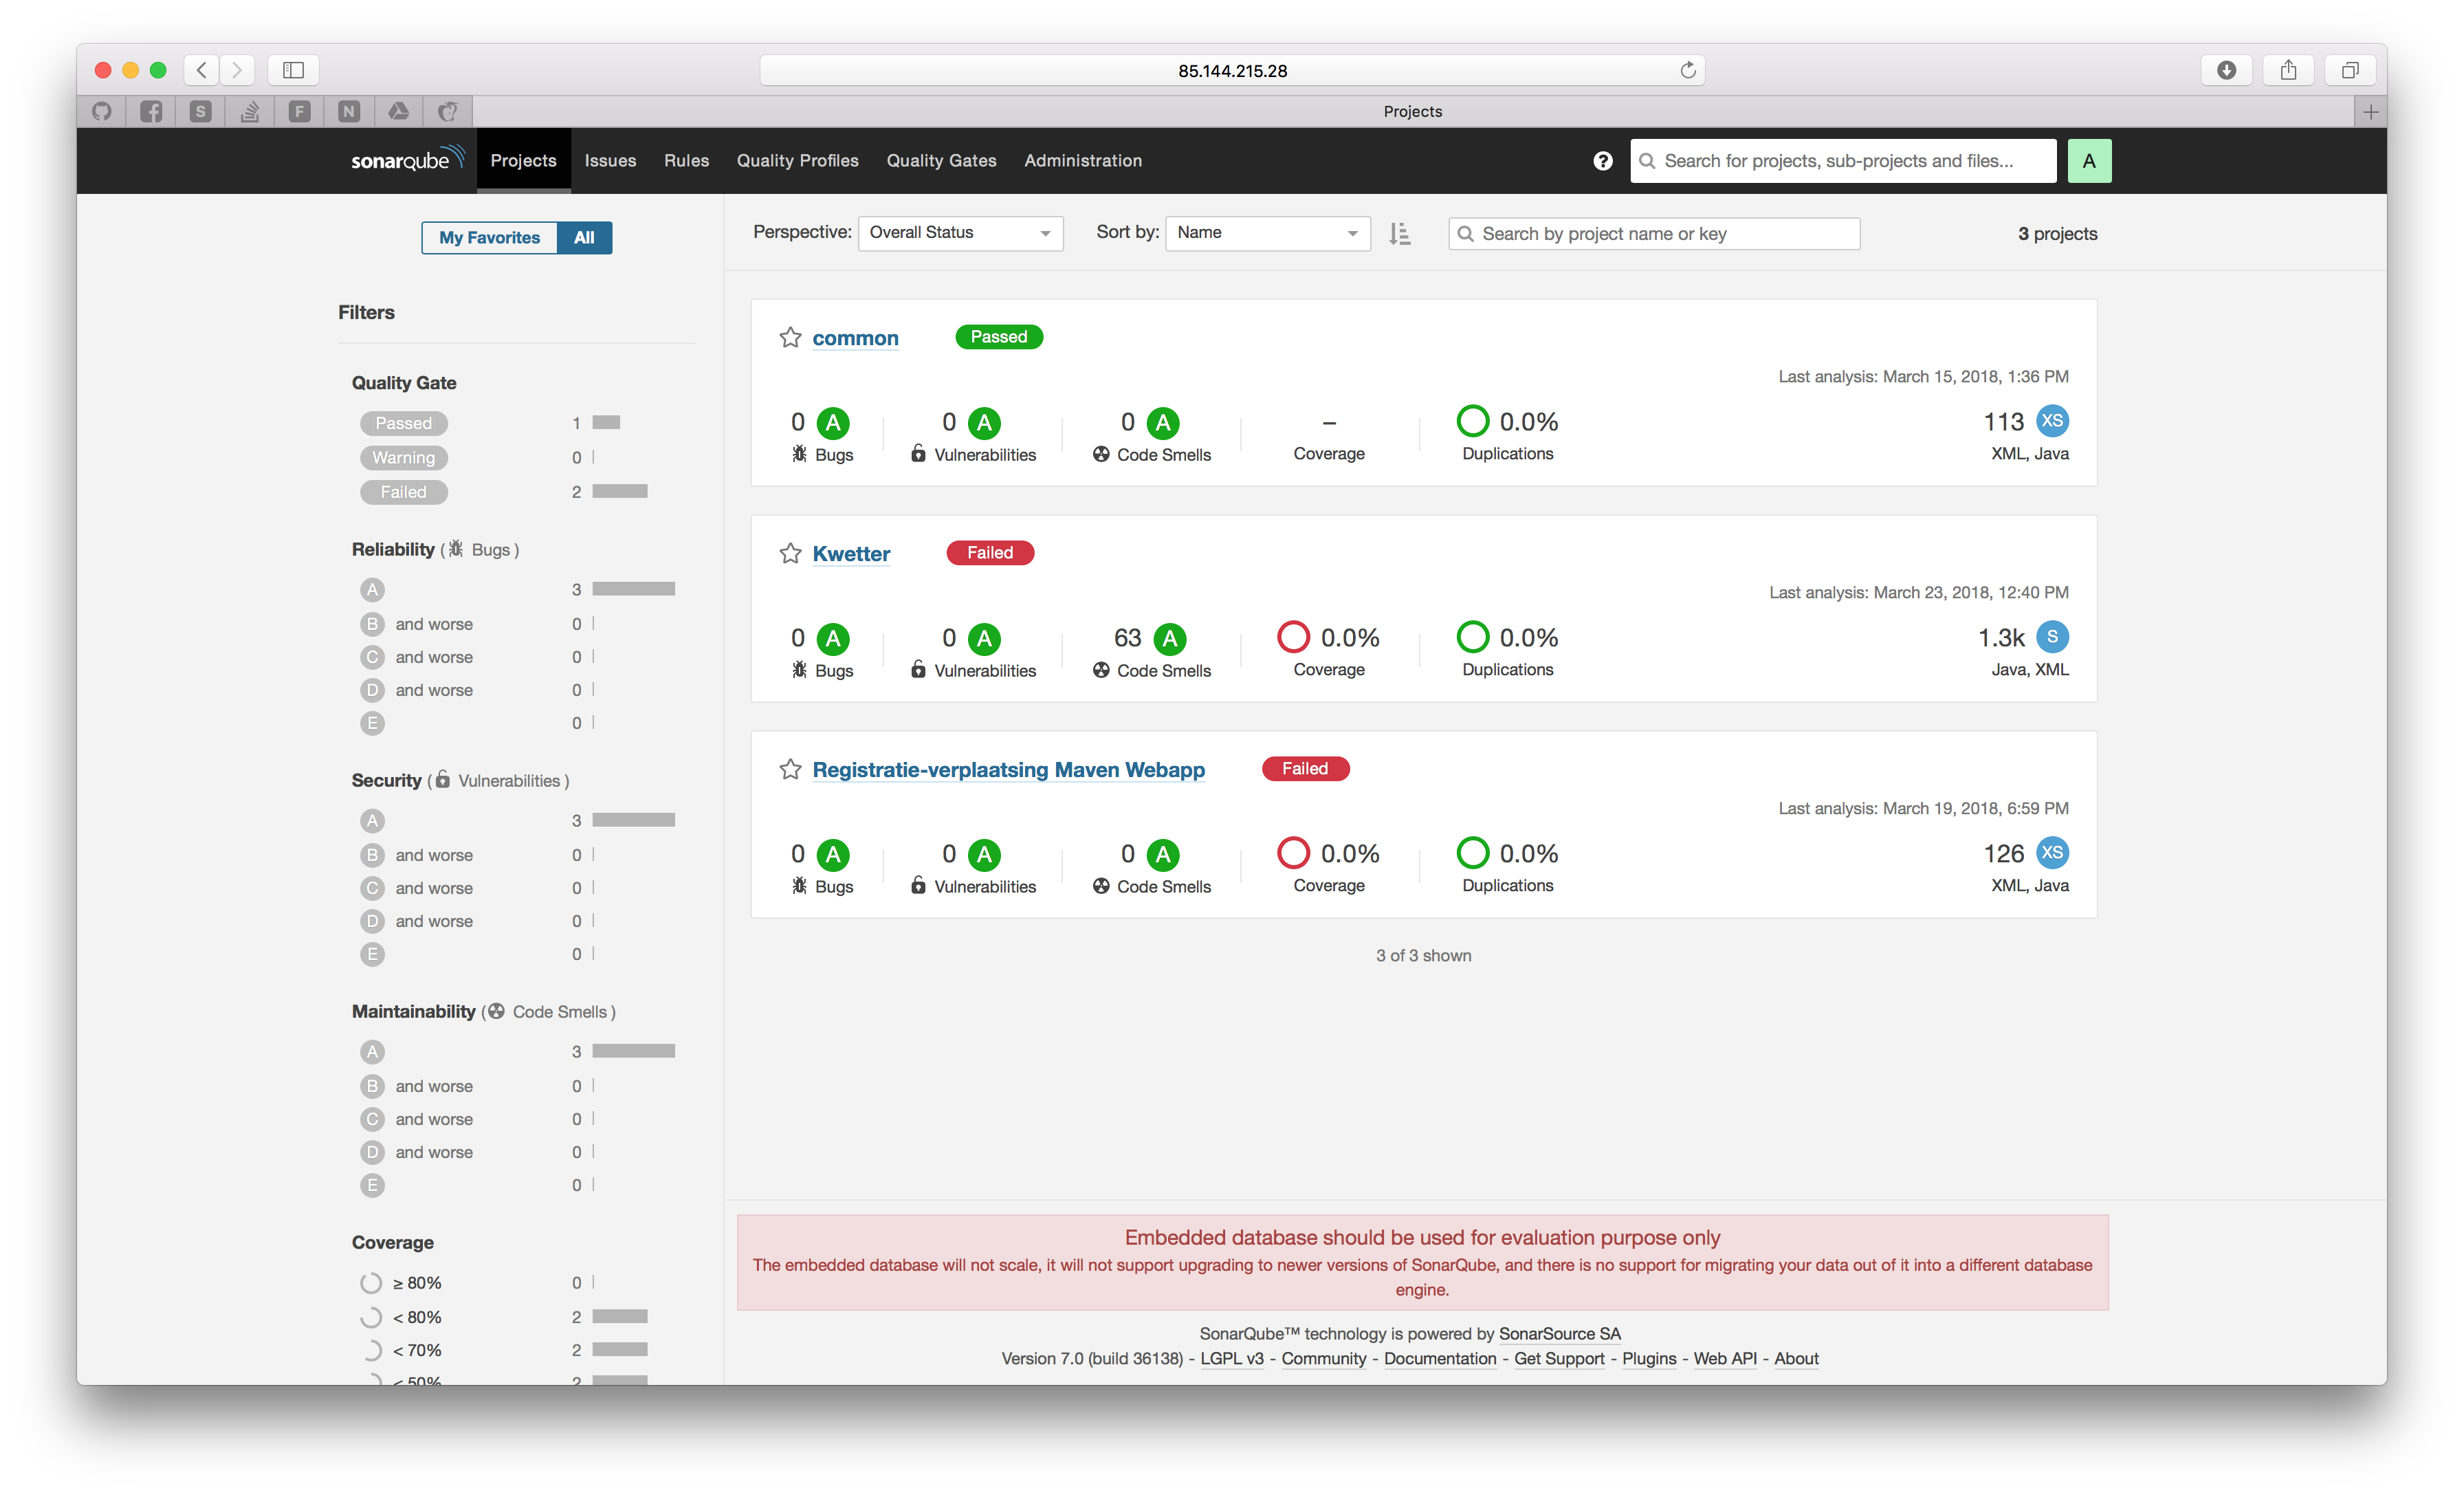
\includegraphics[width=0.95\textwidth]{img/SonarqubeDashboard.png}
	\caption{Sonarqube Dashboard}
	\label{fig:SonarqubeDashboard}
\end{figure}

\subsection{Statistieken}
Wanneer sonarqube de nieuwe code gaat verwerken, worden een aantal statistieken berekent.

\subsubsection{Cyclomatic Complexity}
De Cyclomatische complexiteit die wordt weergegeven door Sonarqube geeft aan hoeveel testcases er nodig zijn om de volledige applicatie te testen (en dus te voorzien van 100\% code coverage).
Op 27 maart is een analyse van één van onze applicaties uitgevoerd. In onderstaande afbeelding geeft de cyclomatische complexiteit weer dat er 101 unit tests nodig zijn om de volledige applicatie te testen.

\begin{figure}[H]
	\centering
	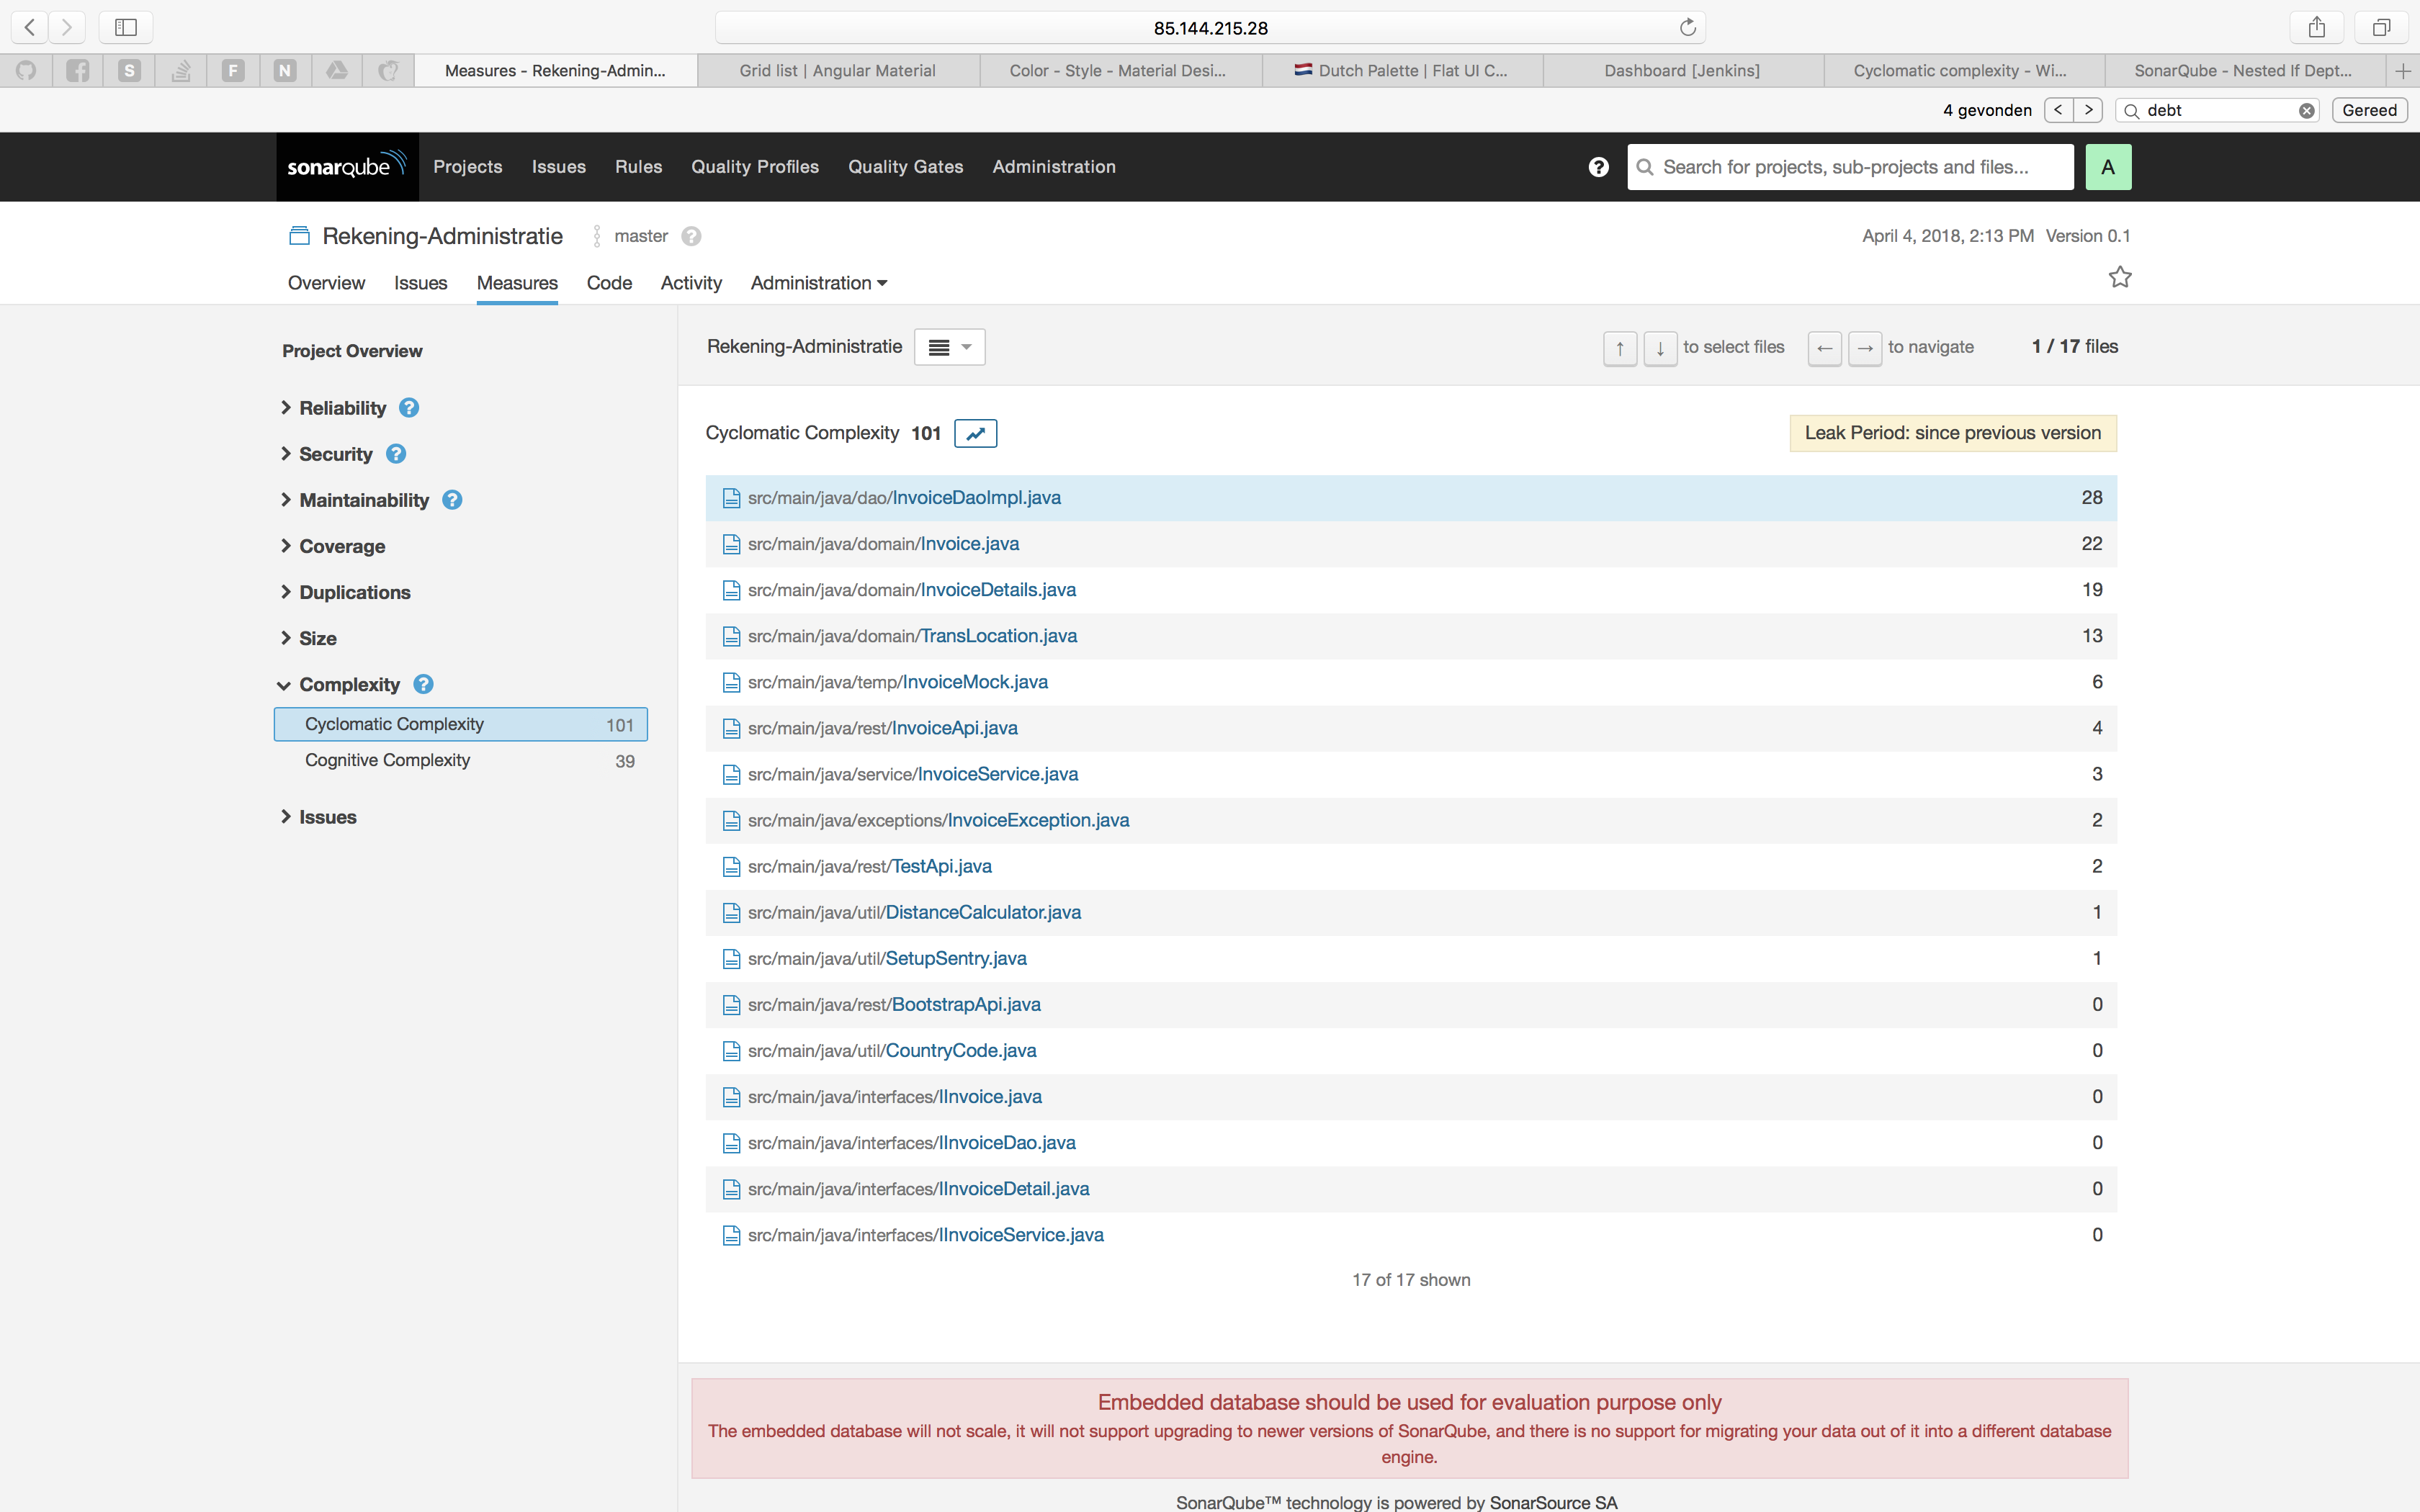
\includegraphics[width=0.95\textwidth]{img/CyclomaticComplexity.png}
	\caption{Cyclomatische complexiteit voor applicatie rekening-administratie in Sonarqube}
	\label{fig:CyclomaticComplexity}
\end{figure}

\subsubsection{Block Depth}
Block debt geeft aan hoevaak statements genest worden (bv. if-statement in if-statement in ...). Dit kan ervoor zorgen dat doe complexiteit van het programma omhoog gaat (ivm code smells).
\subsubsection{Technical debt}
De technical debt geeft aan hoelang het nodig is om code smells van een klasse op te lossen. In onderstaande afbeelding kunnen we zien dat het aantal regels code en de eventuele code smells de benodigde tijd (technical debt) flink kan laten toenemen.

\begin{figure}[H]
	\centering
	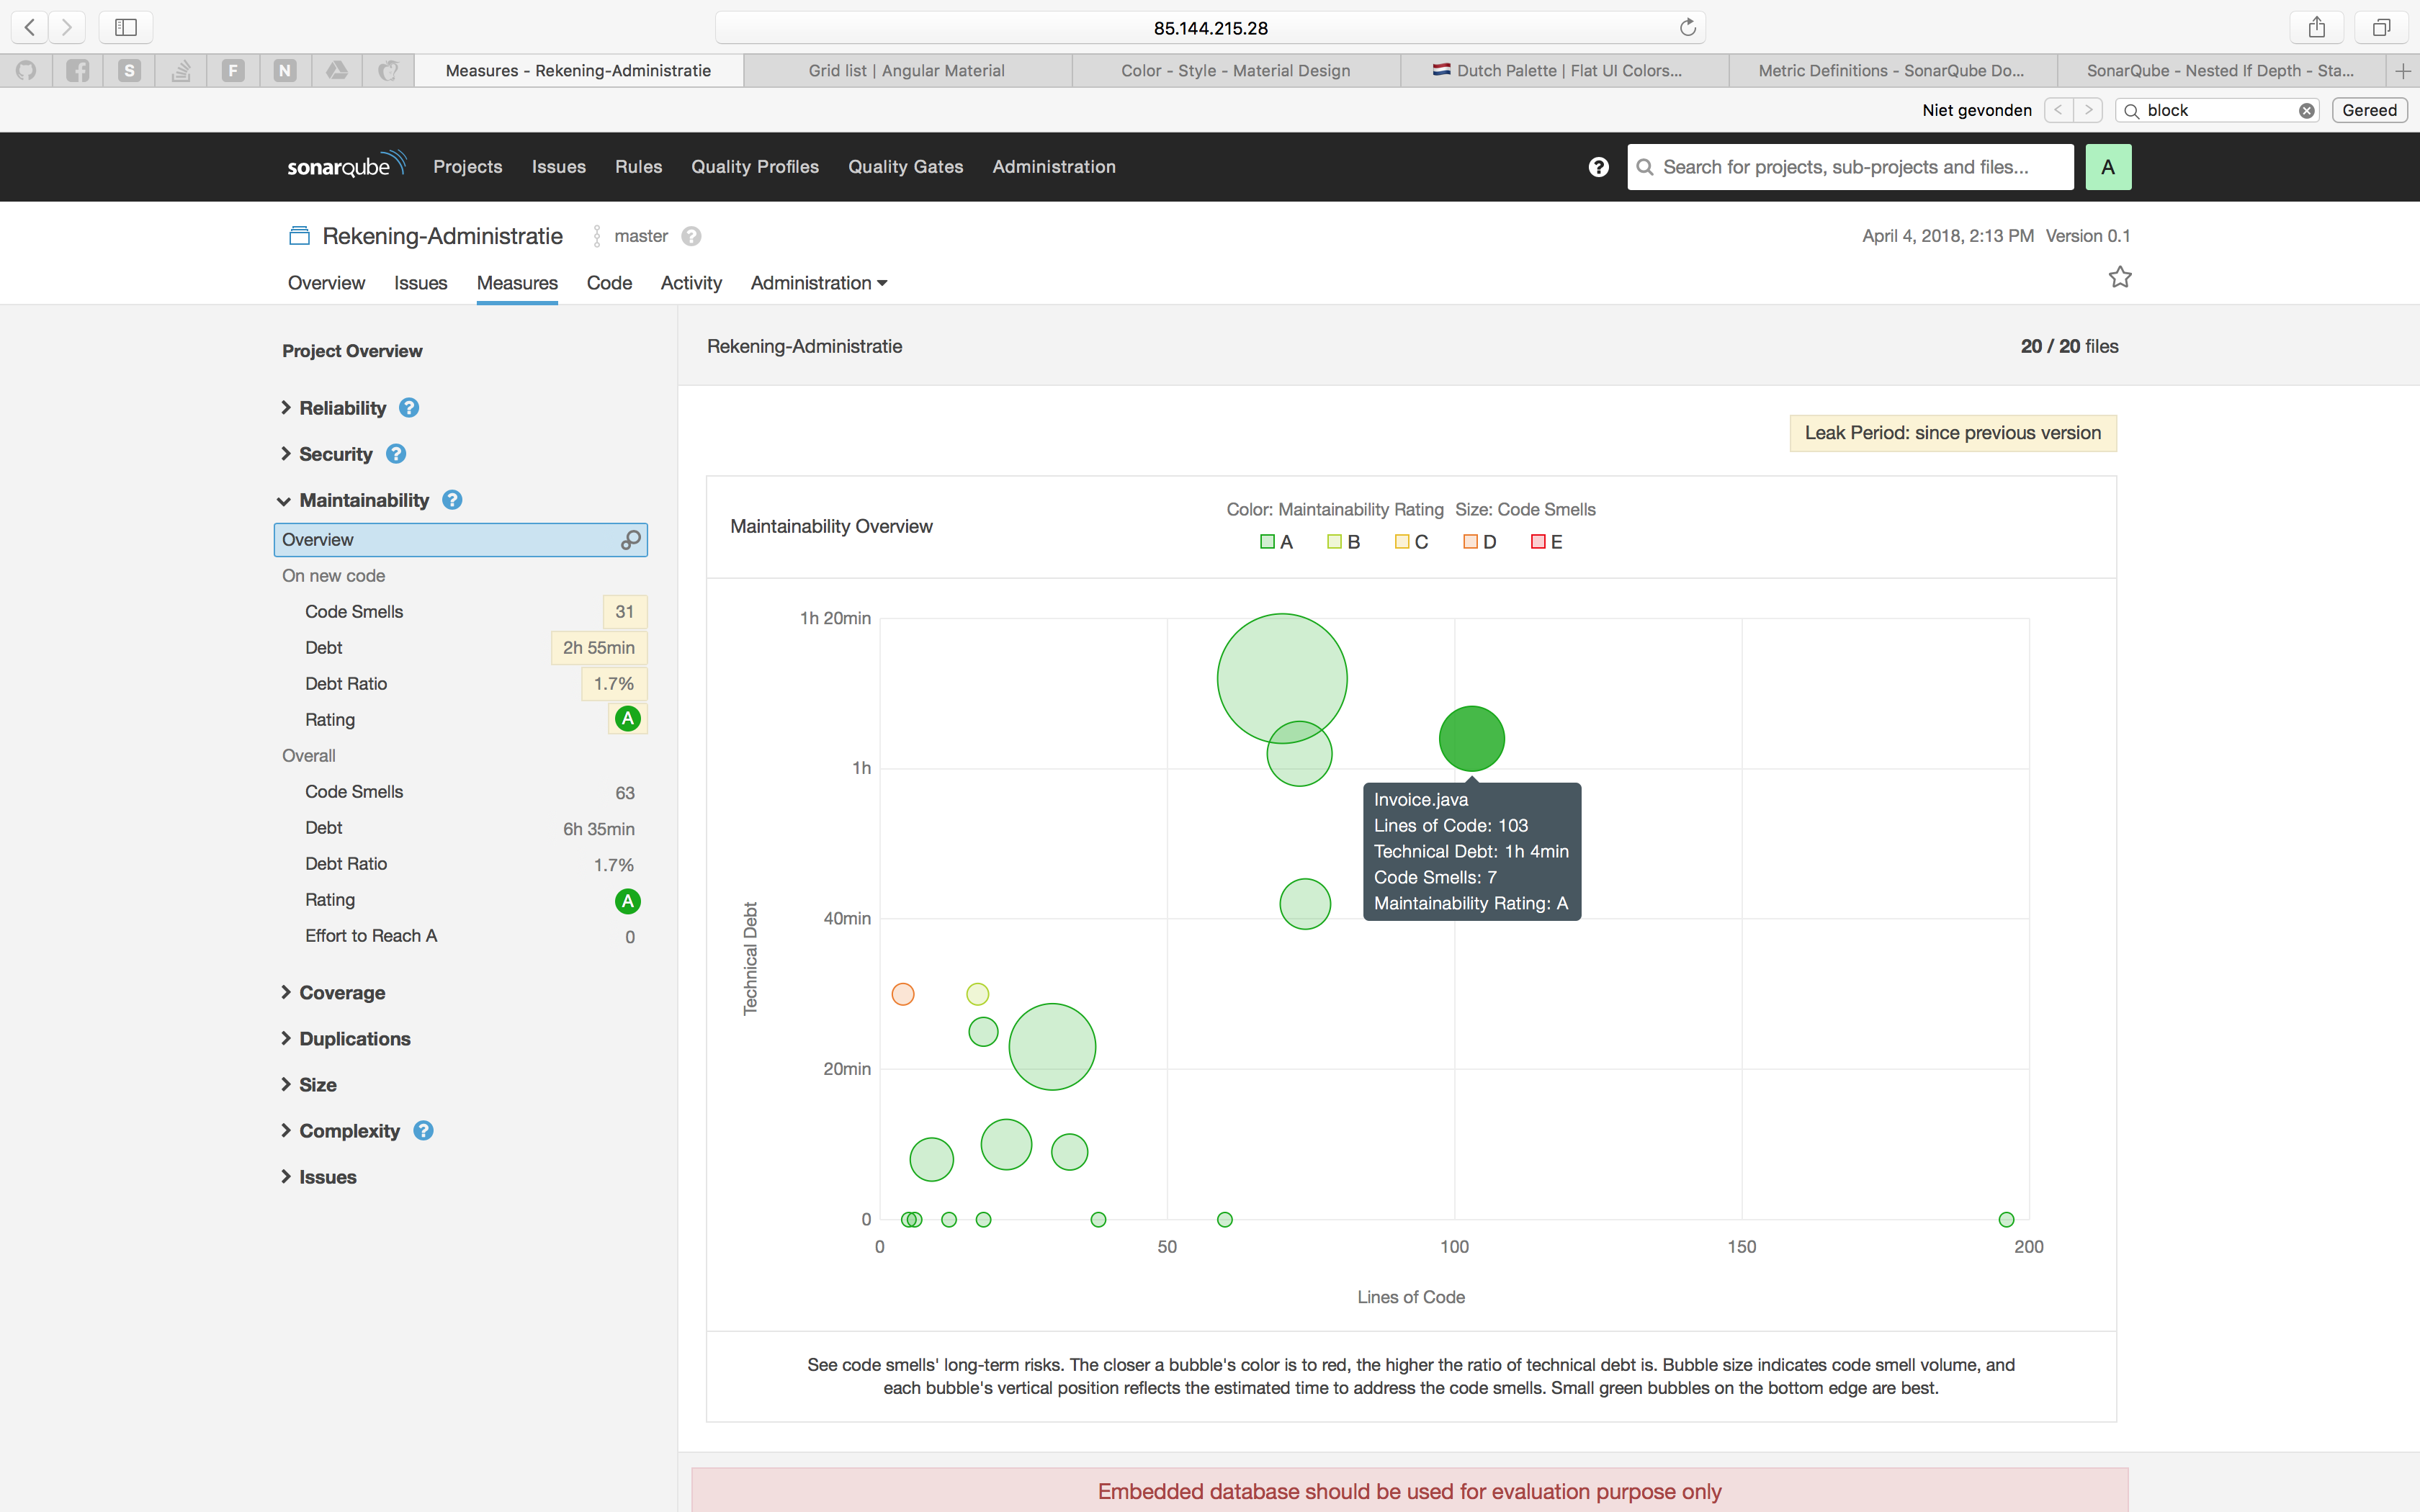
\includegraphics[width=0.95\textwidth]{img/TechnicalDebt.png}
	\caption{Technical Debt van Rekening administratie op 27 maart 2018}
	\label{fig:TechnicalDebt}
\end{figure}
\subsubsection{Fan in/out}
Fan in houdt bij hoeveel methodes een specifieke methode kunnen aanroepen.
Fan out houdt bij hoeveel methodes één specifieke methode kan aanroepen.
\begin{figure}[H]
	\centering
	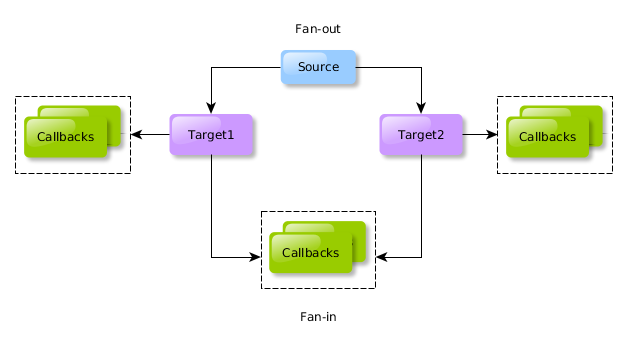
\includegraphics[width=0.95\textwidth]{img/fan-out-fan-in.png}
	\label{fig:faninout}
\end{figure}